\subsection[Мажоритарные генераторы, шифр A5/1]{Мажоритарные генераторы на примере алгоритма шифрования A5/1}

Третий способ улучшения криптостойкости последовательностей поясняется с помощью рис. \ref{fig:gsm-a51-cipher}, на котором показан мажоритарный генератор ключей алгоритма потокового шифрования A5/1 стандарта GSM (GSM-2). В отличие от нелинейного комбинирования выходов нескольких регистров, применен условный сдвиг регистров, то есть на каждом такте некоторые регистры могут не сдвигаться а оставаться в прежнем состоянии. На рисунке показана схема из трех регистров сдвига с различными многочленами обратной связи (здесь применена обратная нумерация ячеек, коэффициентов и переменных по сравнению с предыдущими разделами):
\[ \begin{array}{l}
    c_1(y) = y^{19} + y^{18} + y^{17} + y^{14} + 1; \\
    c_2(y) = y^{22} + y^{21} + 1; \\
    c_3(y) = y^{23} + y^{22} + y^{21} + y^8 + 1.
\end{array} \]

\begin{figure}[h!]
    \centering
	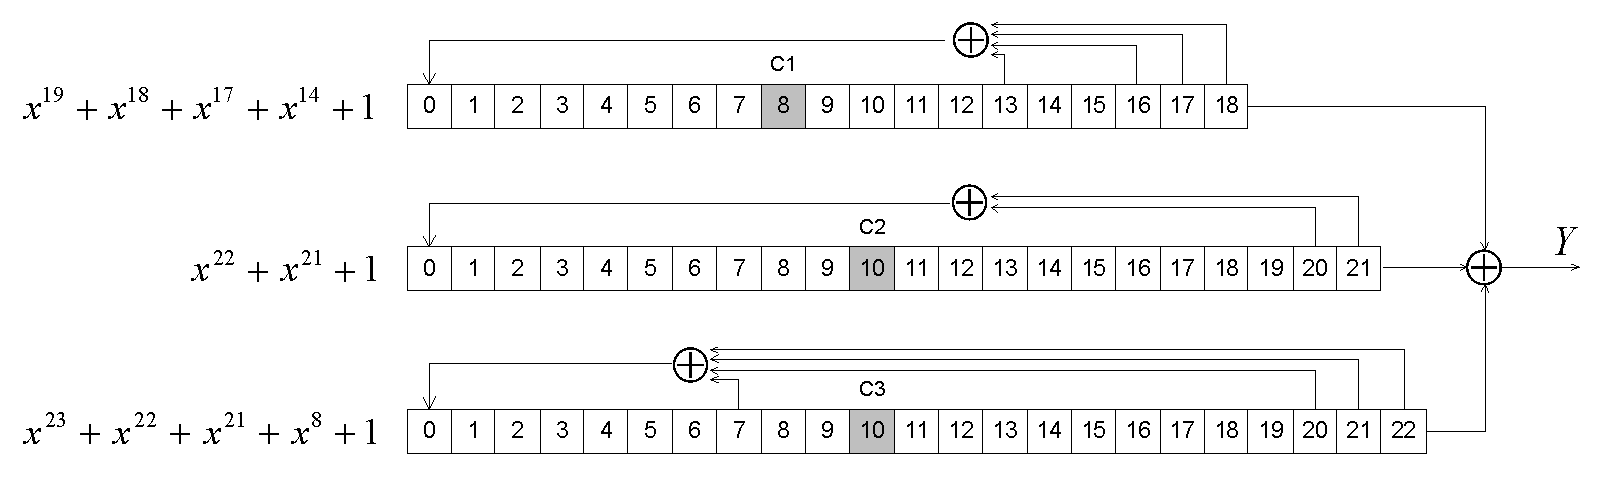
\includegraphics[width=\textwidth]{pic/gsm-a51-cipher}
    \caption{Регистр сдвига алгоритма шифрования A5/1\label{fig:gsm-a51-cipher}}
\end{figure}

В алгоритме A5/1 регистры сдвигаются не на каждом такте. Правило сдвига следующее. В каждом регистре есть один тактовый бит, определяющий сдвиг  -- восьмой бит $\textrm{C1}$ для первого регистра, и десятые биты $\textrm{C2}$ и $\textrm{C3}$ для второго и третьего регистров. На каждом такте вычисляется мажоритарное значение тактового бита $m = \textrm{majority}(\textrm{C1}, \textrm{C2}, \textrm{C3})$, т.е. по большинству значений: 0 или 1. Если для данного регистра значение тактового бита совпадает с мажоритарным решением, то регистр сдвигается. Если не совпадает, остается в прежнем состоянии без сдвига на следующий такт. Так как всего состояний тактовых битов $2^3$, то в среднем каждый регистр сдвигается в $\frac{3}{4}$ всех тактов.

Общее количество ячеек всех трех регистров $19+22+23=64$, следовательно, период генератора A5/1 ~ $T < 2^{64}$. Данный шифр не может считаться стойким из-за возможности полного перебора. Например, известны атаки на шифр A5/1, требующие 150-300 GiB оперативной памяти и нескольких минут вычислений одного ПК (2001 г.).
